\documentclass[10pt,a4paper,oneside,abstracton]{scrartcl}
\usepackage[utf8]{inputenc}
\usepackage[english, ngerman]{babel}
% \usepackage{underscore}

\usepackage{gensymb}

\usepackage{amsmath}
\usepackage{amsfonts}
\usepackage{amssymb}
\usepackage{graphicx}
\usepackage{lmodern}
	%\usepackage{kpfonts}
\usepackage{fourier}
\usepackage[left=2cm,right=2cm,top=2cm,bottom=2cm]{geometry}
\usepackage{multicol}
\setcounter{secnumdepth}{4} %Nummerierungstiefe bis Paragraph (4. Ebene)
\usepackage{blindtext}
\usepackage[ 		%Einstellungen für Link
   colorlinks,        % Link ohne Umrandungen in zu wählender Farbe 
   linkcolor=black,   % Farbe interner Verweise 
   filecolor=black,   % Farbe externer Verweise 
   citecolor=black    % Farbe von Zitaten 
]{hyperref}



\newenvironment{Figure}
  {\par\medskip\noindent\minipage{\linewidth}}
  {\endminipage\par\medskip}


\pagestyle{empty}		%Seitenzahl wird nich angezeigt

\begin{document}

\section*{Praktische Anwendung einer elektrischen und thermischen Simulation einer Platine zur Ansteuerung eines BLDC-Motors}
\section*{Christian Schmid}
Hochschule Augsburg, Fakultät für Elektrotechnik, Augsburg, Deutschland, Christian.Schmid1@Hs-Augsburg.de 


\begin{abstract} %kann man auch ueber /subsection machen
\noindent %einrücken verhindern
Dies ist ein normaler Text in 10 pt Schriftgröße und 12 pt Zeilenabstand. Dies ist ein normaler Text in 10 pt Schriftgröße und 12 pt Zeilenabstand. Dies ist ein normaler Text in 10 pt Schriftgröße und 12 pt Zeilenabstand. Dies ist ein normaler Text in 10 pt Schriftgröße und 12 pt Zeilenabstand. Dies ist ein normaler Text in 10 pt Schriftgröße und 12 pt Zeilenab-stand. Dies ist ein normaler Text in 10 pt Schriftgröße und 12 pt Zeilenabstand. Dies ist ein normaler Text in 10 pt Schriftgröße und 12 pt Zeilenabstand. Dies ist ein normaler Text in 10 pt Schriftgröße und 12 pt Zeilenabstand. Dies ist ein normaler Text in 10 pt Schriftgröße und 12 pt Zeilenabstand.
\end{abstract}

\renewcommand{\abstractname}{Abstract} %aendert name Zusammenfassung in Abstract

\begin{abstract}
\noindent %einrücken verhindern
Dies ist ein normaler Text in 10 pt Schriftgröße und 12 pt Zeilenabstand. Dies ist ein normaler Text in 10 pt Schrift-größe und 12 pt Zeilenabstand. Dies ist ein normaler Text in 10 pt Schriftgröße und 12 pt Zeilenabstand. Dies ist ein normaler Text in 10 pt Schriftgröße und 12 pt Zeilen-abstand. Dies ist ein normaler Text in 10 pt Schriftgröße und 12 pt Zeilenabstand.
\end{abstract}


\begin{multicols}{2}
\section{Grundlagen}
\subsection{Thermische Auslegung}
Eletrische Komponenten haben einen Temperaturbereich. 
Bauteile werden von dem Hersteller getestet und haben in diese Temperaturbereich einen von Hersteller angegebenen Lebenszyklus. 
Bei überschreiten der Temperatur kann die Lebenszeit der Bauteile rapide abnehmen. 
Besonders gefährdet sind Elektrolyt Kondensatoren. 
Die maximale Temperatur beträgt meist $ 105 \degree C $. \newline
Bei unterschreiten der maximalen Temperatur um $ 10K $ verdoppelt sich die Lebenszeit. 
Alle $ 10K $ weniger verdoppelt sich der Lebenszyklus \cite{Elko}. 
\newline
Um die Verluste und daraus entstehende Abwärme durch Selbstinduktion und elektrische Widerstände  auf der Leiterbahn gering zu halten,
wird die Leiterbahn abhängig von der Anwendung unterschiedlich ausgelegt.
\newline
Eine Versorungsleitung benötigt eine größere Leiterbahnfläche als eine Messleitung, da die Versorungsleitung einen höheren Strom führt. 

\subsection{BLDC-Motor Aussteuerung}
Der Brushless DC Motor ist eine Synchronmaschine. 
Eine Synchronmaschine braucht 3 zueinander versetzte Phasen mit Spannungen, die einen sinus darstellen.
Um die Funktionsweise zu erhalten wird das Stellglied getaktet an und abgeschaltet. 
Die Schaltfrequenz ist 100 - 10.000 so groß wie die gewollte Winkelgeschwindigkeit. 
Die Schaltfrequenz ist zu groß für das System. (vgl. Abbildung \ref*{Aussteuerung})
\newline
Es stellt sich eine mittlere Spannung ein, die sich über der Zeit nur langsam verändert.
Das System folgt der dem Sollsignal.

\begin{Figure}
	% \resizebox{0.1\columnwidth}{!} 
	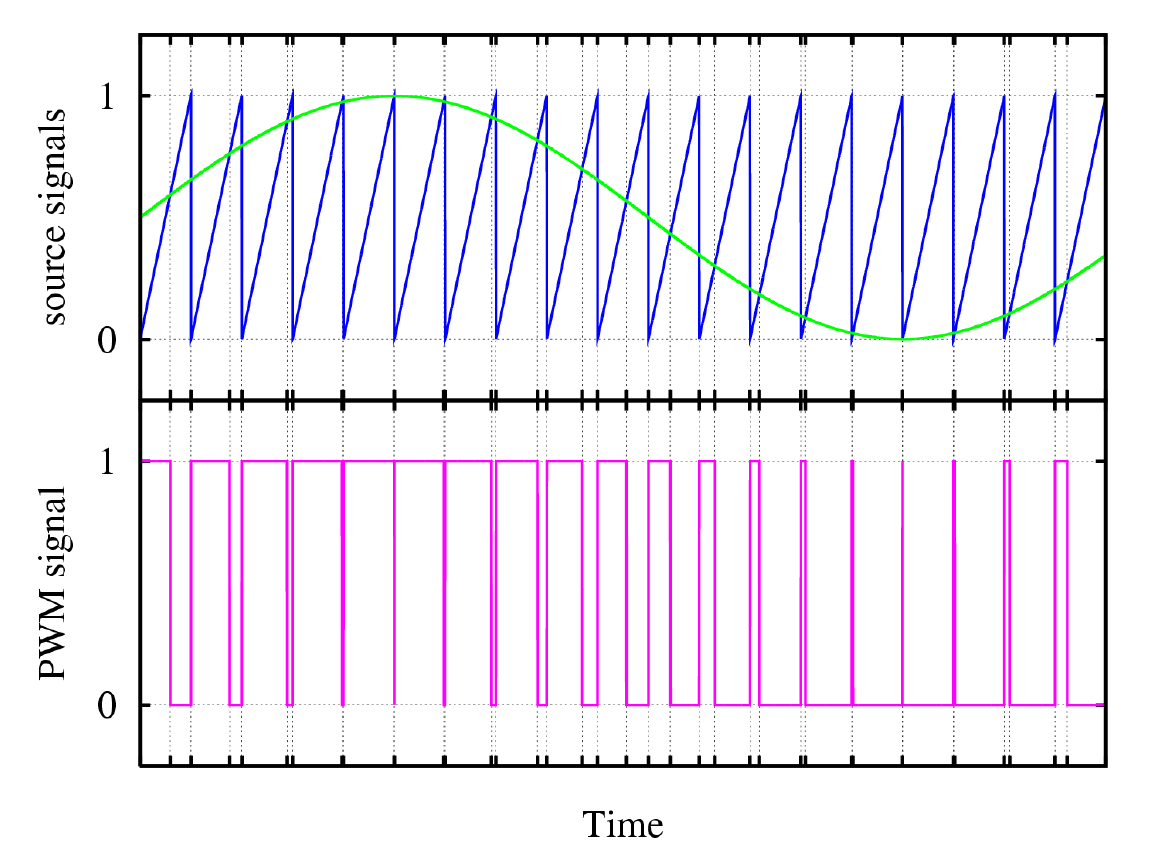
\includegraphics[width=\textwidth]{Bilder/BLDC_Aussteuerung.png}
	\captionof{figure}{Aussteuerung einer Phase}
	\label{Aussteuerung}
\end{Figure}

\noindent
Die Schematische Funktionsweise eines Brushless DC Motors sieht wie folgt aus. 
Mittels 3 Halbbrücken werden die drei Phasen des Motors getrennt angesteuert und der Motor gesteuert, 
beziehungsweise geregelt(vgl. Abbildung \ref*{Motor_Schematic}). 
Die Geschwindigkeit wird vorgegeben, indem die Winkelgeschwindigkeit $ \omega $ eingestellt wird. 
 $ \omega = 2\pi \cdot n = \frac{d\varphi}{dt} $   
 \newline
Die Spulenspannung wird durch $ u(t) = U \cdot sin(\omega \cdot t + \varphi_U) $ eingestellt. 
\begin{Figure}
	% \resizebox{0.1\columnwidth}{!} 
	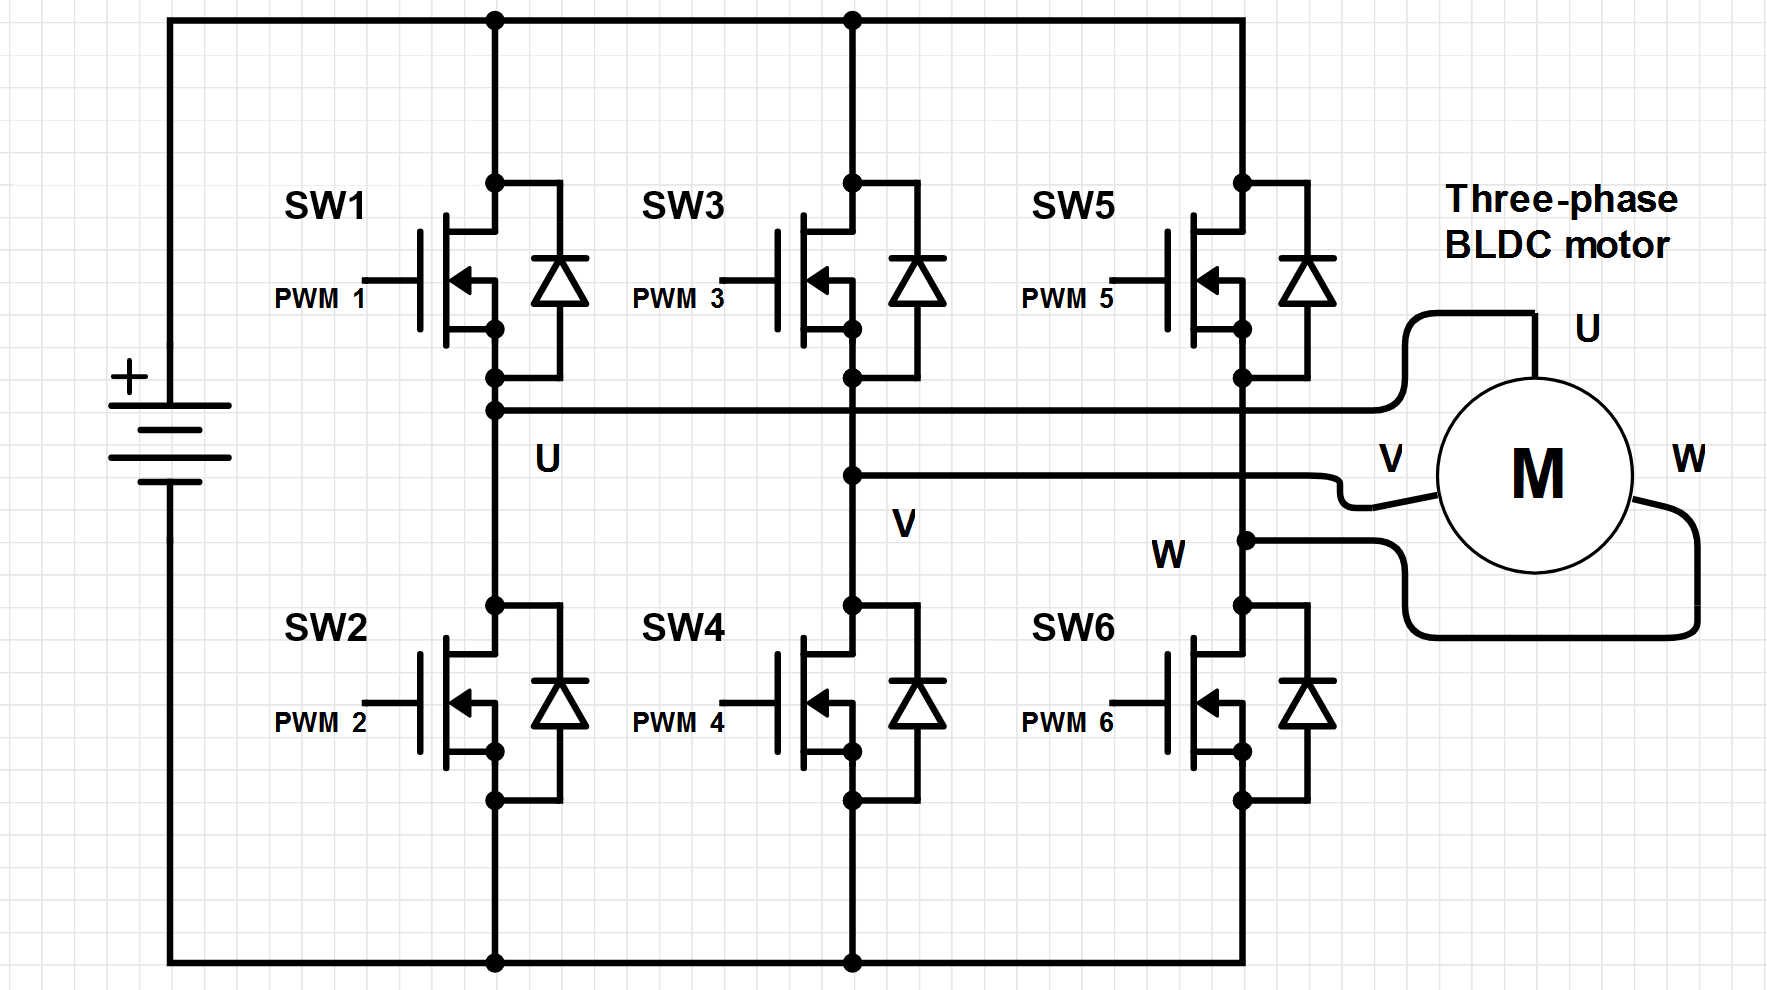
\includegraphics[width=\textwidth]{Bilder/BLDC_Schematic.png}
	\captionof{figure}{Schematische Funktionsweise eines BLDC Motors \cite{Motor_Ansteuerung}}
	\label{Motor_Schematic}
\end{Figure}

\subsubsection{Folgerung}
Da sich der eingestellte Strom sehr schnell verändert und das Thermische System langsamer ist als die Motoransteuerung, 
kann davon ausgegangen werden, dass in den Leitungen ein konstanter Strom fließt. 
Es wird angenommen dass bei maximalem Drehmoment ein Strangstrom von bis zu $I_{Strang} = 5 A $  fließt. 

\section{Thermisches Desgin}
Abhängig von dem einstellten Strom gibt es in der Industrie vorgaben, wie breit Leiterbahnen sein sollen.
Für einen Strom von $I_{Strang} = 5 A $ und einer maximalen Erwärmung von $10 K$ ergibt sich eine
Leiterbahnbreite von $b = 4 mm $.

\subsection*{Aufbau einer Platine}
Der Aufbau einer 2 lagigen Platine ist in Abbildung \ref*{pcb_im} dargestellt. 
\newline
Die mittlere Schicht der Platine besteht aus einem $ 1,5mm $ breiten Dielektrikum \cite{PCB_Querschnitt}. 
\newline
Die Breite der Leiterbahnen betragen $ 35 \mu m$ auf Ober- und Unterseite \cite{aisler}.


\begin{Figure}
	% \resizebox{0.1\columnwidth}{!} 
	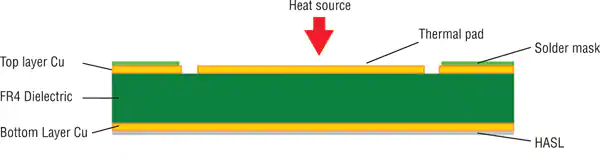
\includegraphics[width=\textwidth]{Bilder/PCB_Querschnitt.png}
	\captionof{figure}{Schematische Funktionsweise eines BLDC Motors \cite{PCB_Querschnitt}}
	\label{pcb_im}
\end{Figure}

 \subsection*{Überprüfung des Vorgabewerts}
Diese Arbeit widmet sich dem Ausrechnen des Thermischen Widerstands und der 
Platinenerwärmung durch den eingestellten Strom. 

\subsection*{Wärmestrom}
Der Wärmestrom wird durch den elektrischen Strom durch die Leiterbahn bestimmt. 
\newline
Die elektrische Leitfähigkeit beträgt:  $ \rho = \frac{58.1e6}{Sm^{-1}} $
Die Fläche der Leiterbahn beträgt: 
\begin{equation}
	R_{Leiter} = \frac{1}{\rho} \cdot \frac{l}{A}
\end{equation}

\subsection*{Daumenregel}
Eine einfache Näherung um die Erwärmung zu bestimmen




\begin{Figure}
	% \resizebox{0.1\columnwidth}{!} 
	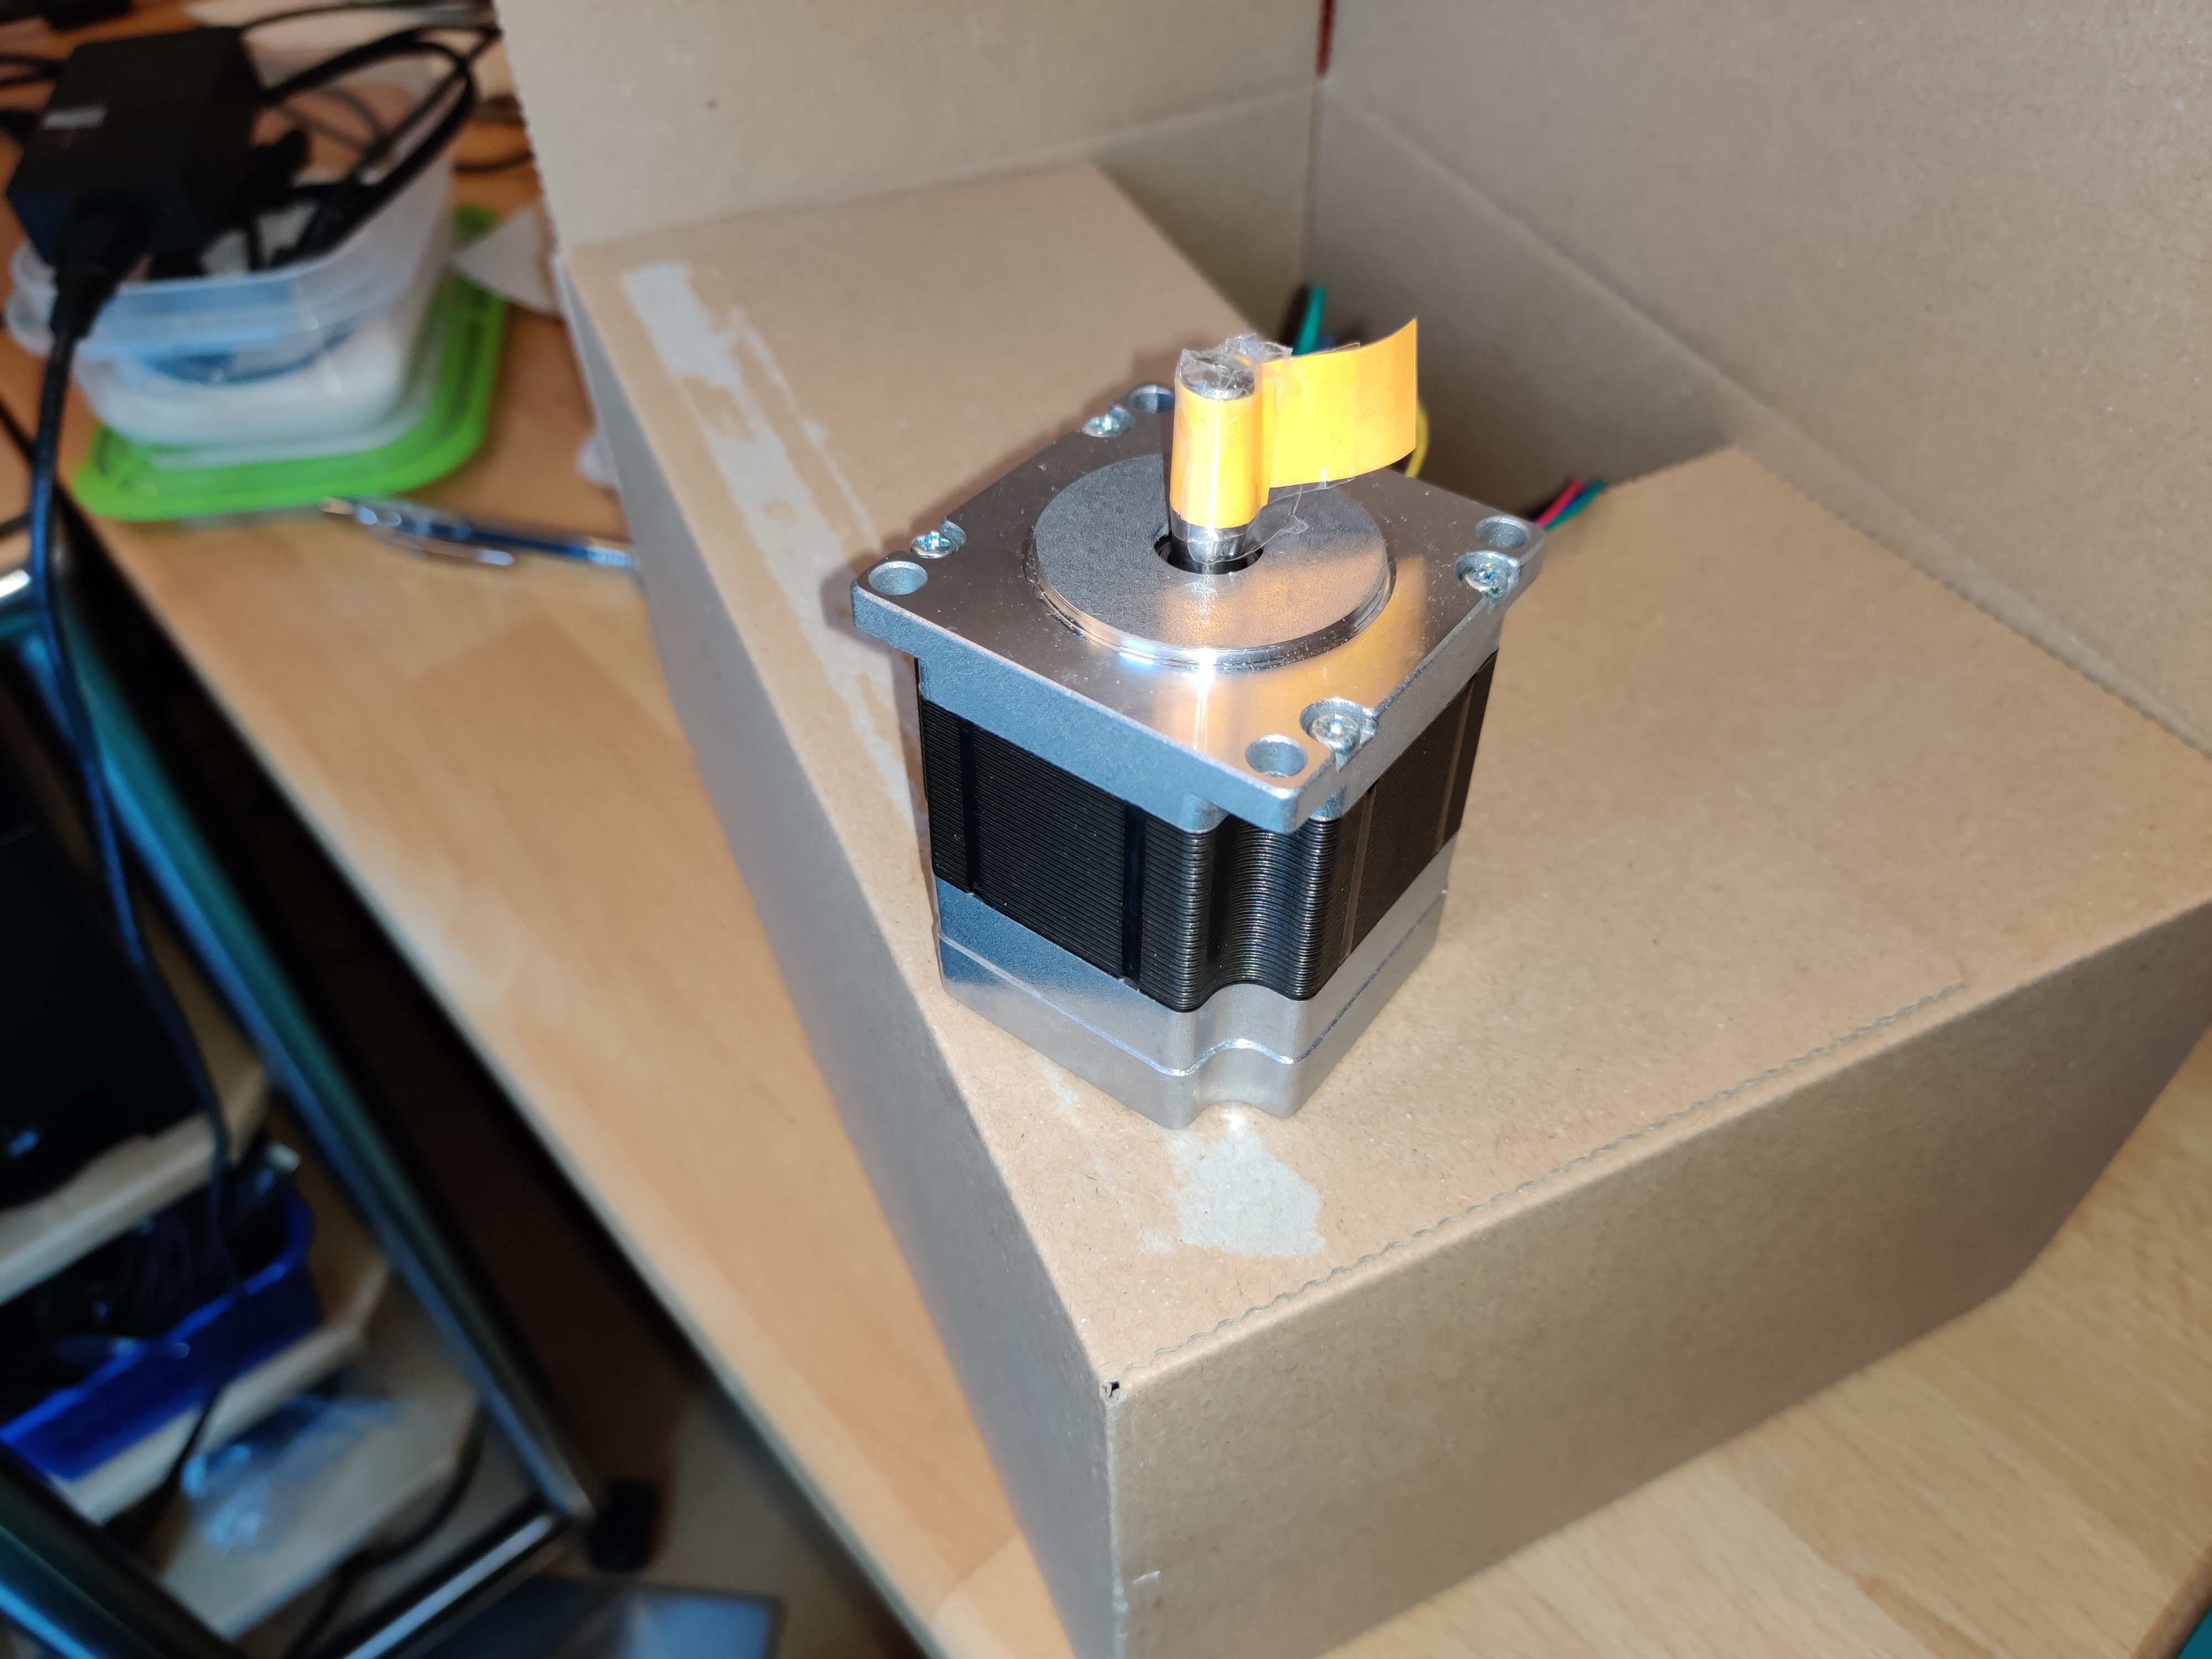
\includegraphics[width=\textwidth]{Bilder/BLDCMotor.jpg}
	\captionof{figure}{my caption of the figure 	\cite{Abramo80}}
\end{Figure}

\section{}
% \begin{minipage}
% 	% 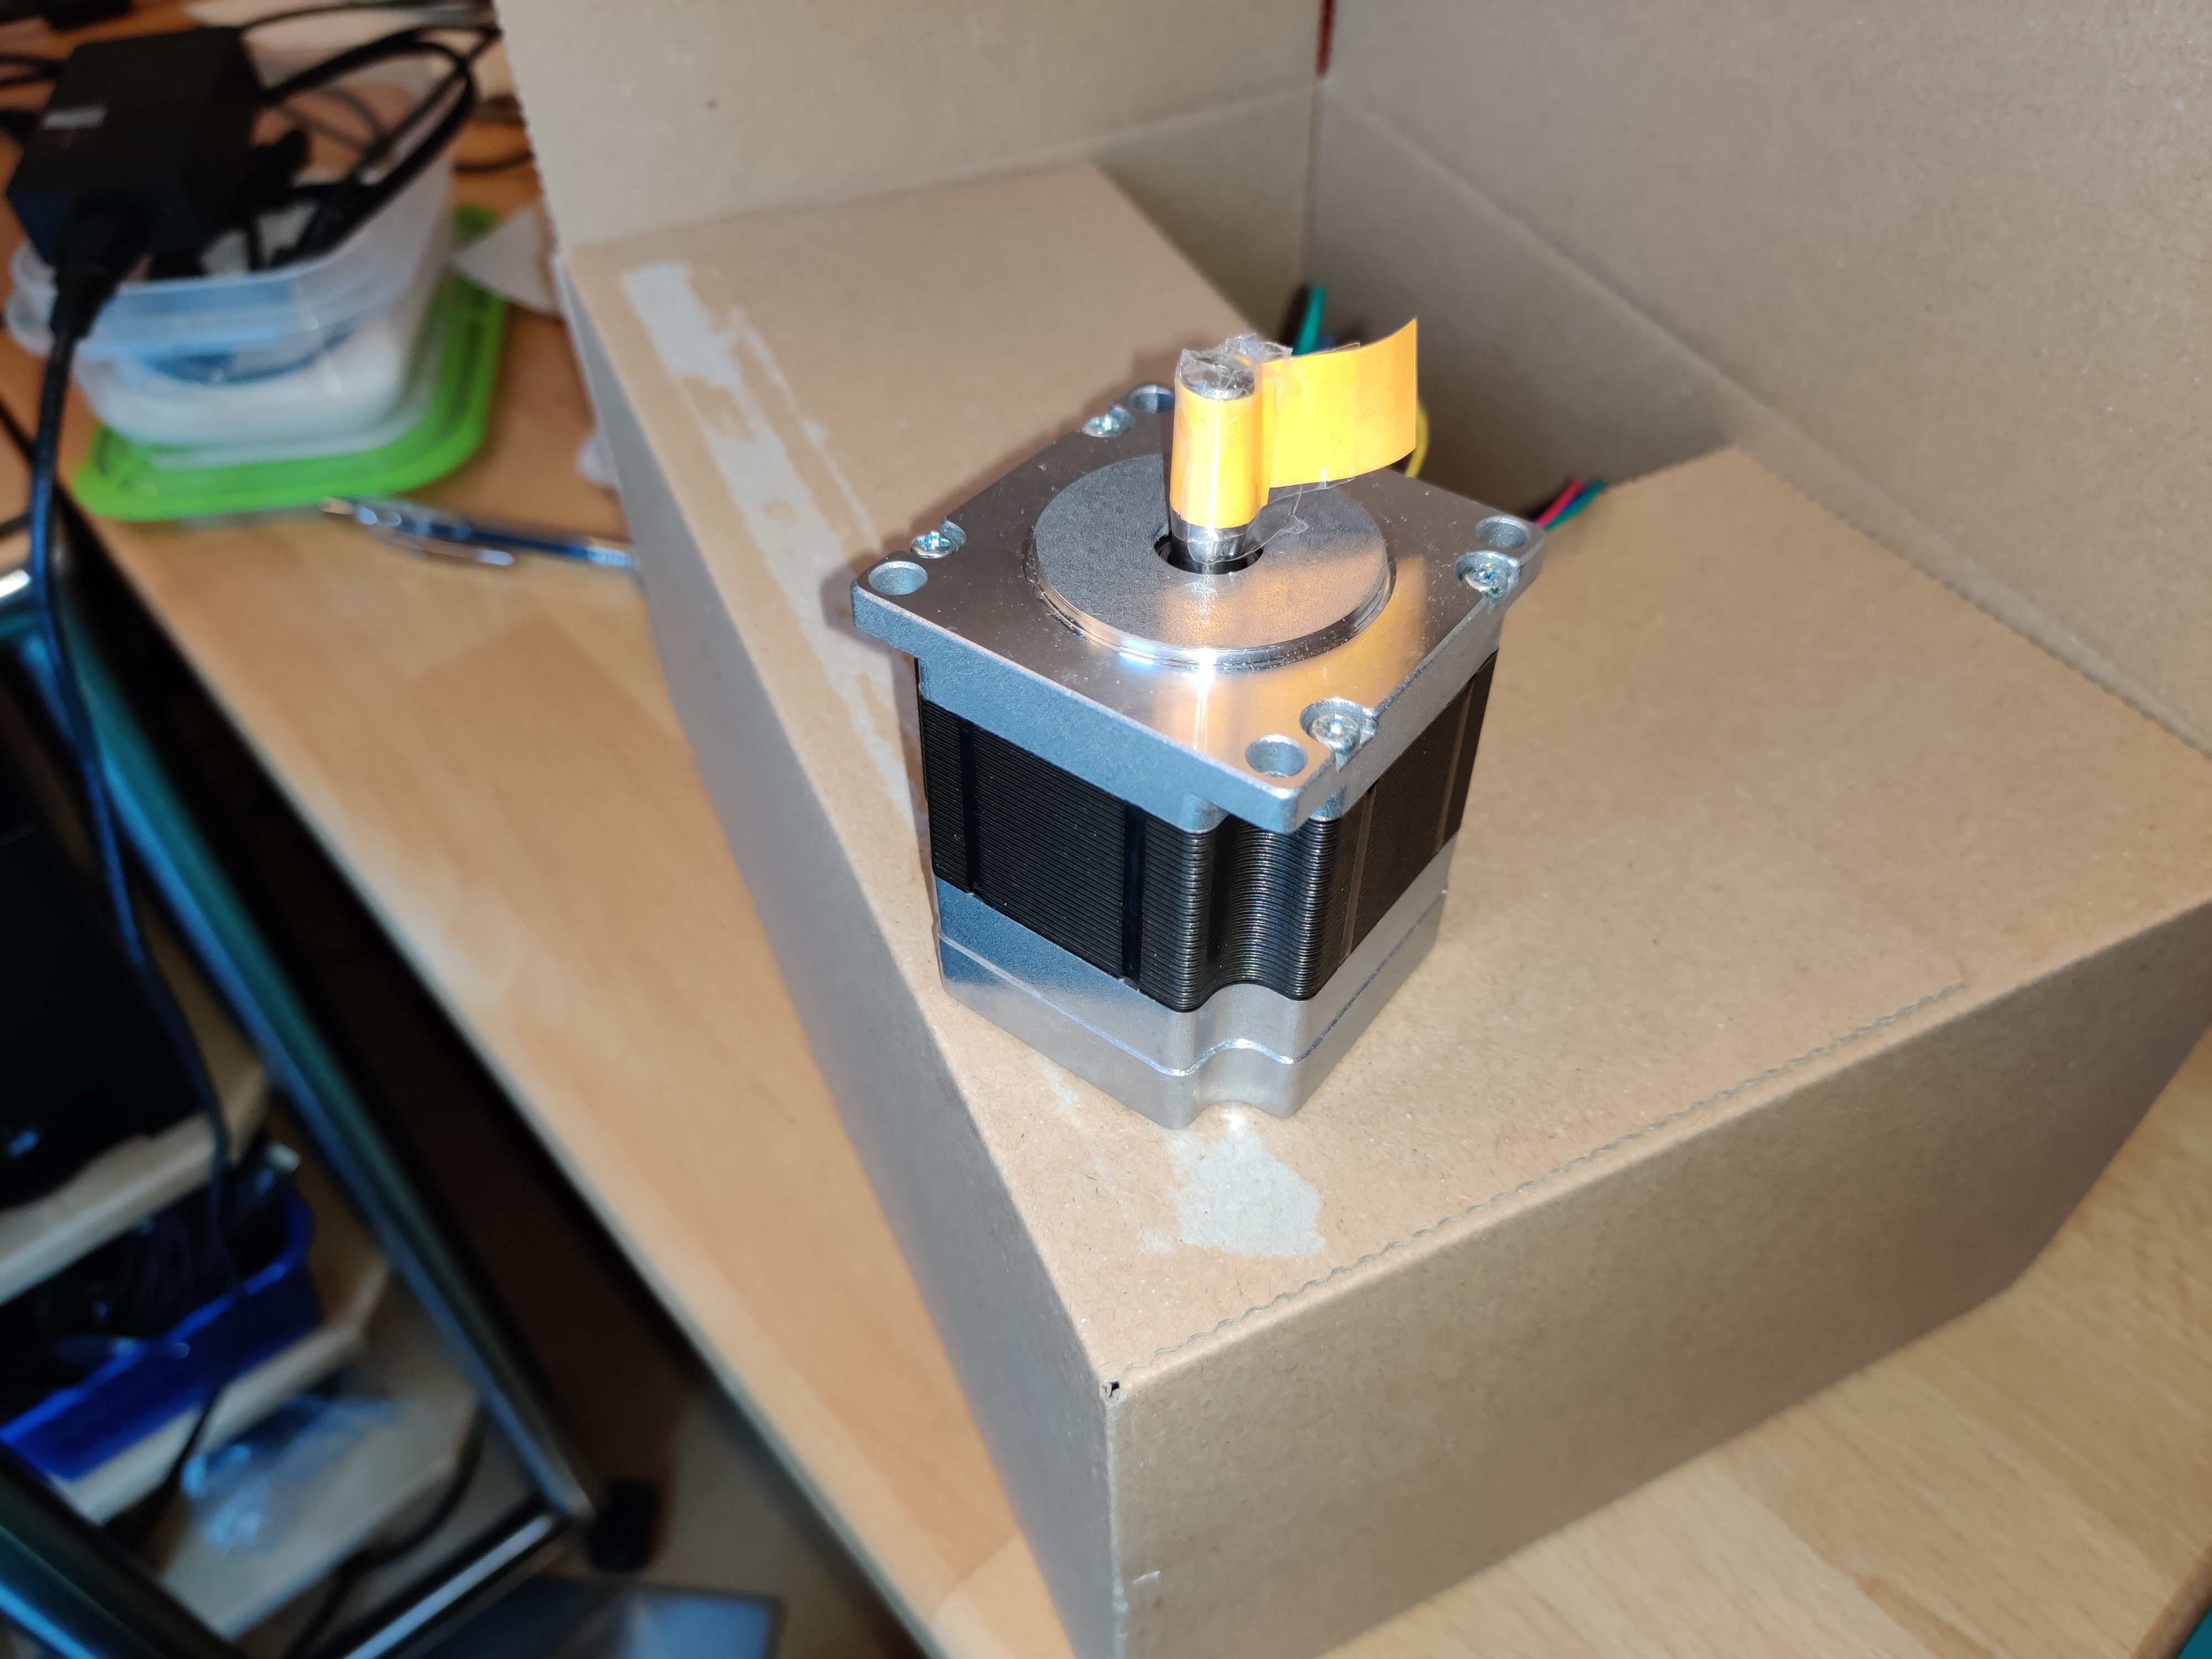
\includegraphics{Bilder/BLDCMotor.jpg}
% \end{minipage}

test
% \newline
% \noindent%
% \begin{minipage}{0.9\columnwidth}  %.9 auf 90 Prozent skaliert 
% \centering 
% \resizebox{0.9\columnwidth}{!} 
% 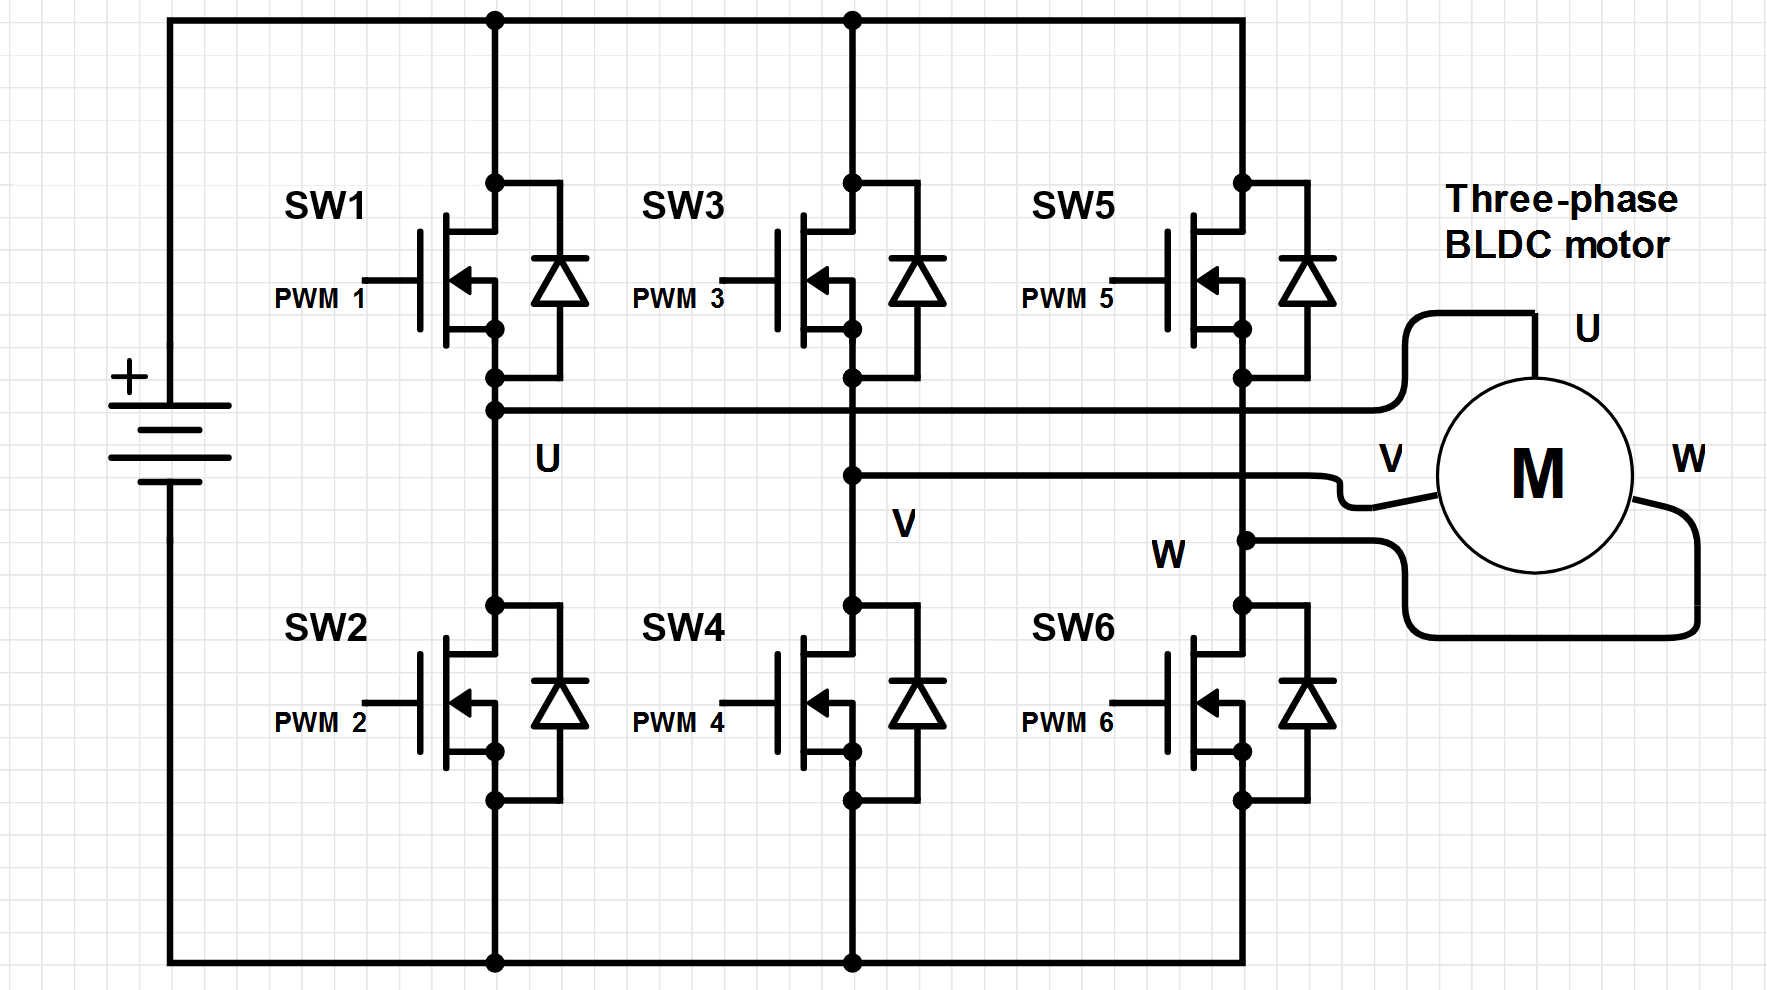
\includegraphics[width=\textwidth]{./Bilder/BLDC_Schematic.png} 
% % \captionof{figure}[Kurz-Caption]{Ansteuerung eines BLDC Motors in Abhängigkeit von Hall Signalen \label{caption} \cite{Motor_Ansteuerung}} 
% \end{minipage} 
% \vspace{4mm}
% \hspace{-4mm}

% % test
% % \newline
% \noindent%
% \begin{minipage}{0.9\columnwidth}  %.9 auf 90 Prozent skaliert 
% \centering 
% \resizebox{0.9\columnwidth}{!} 
% 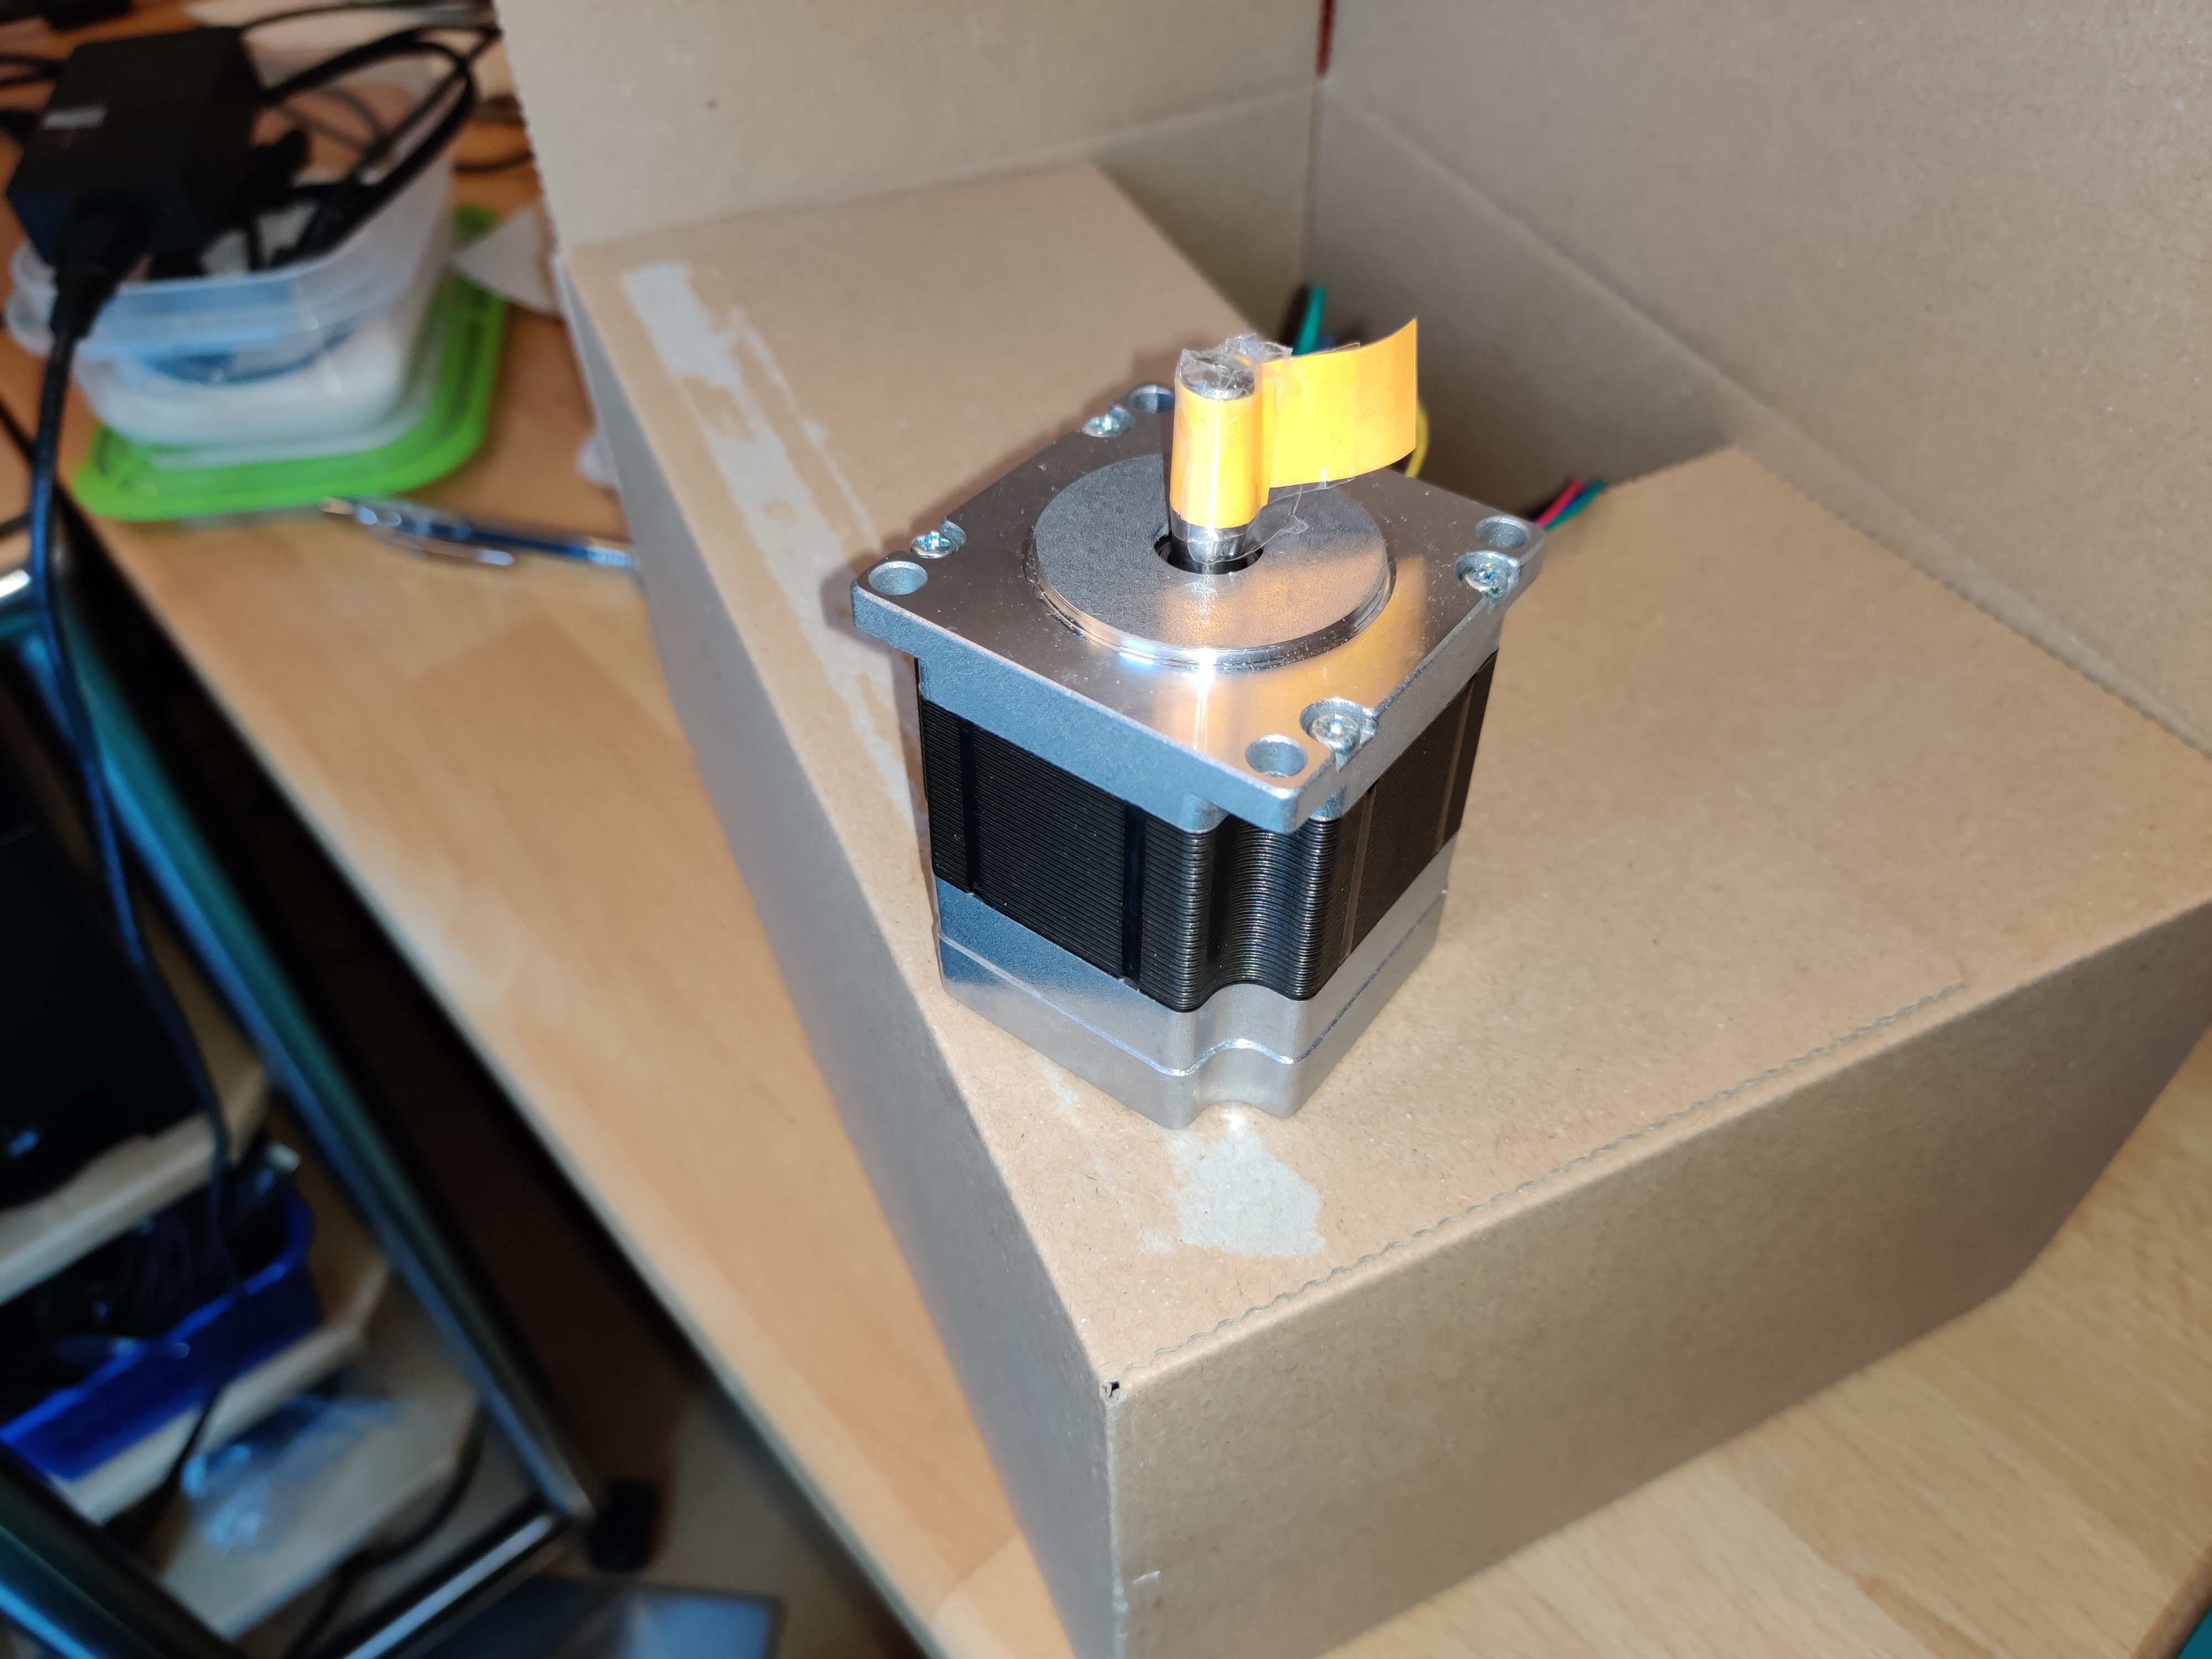
\includegraphics[width=\textwidth]{Bilder/BLDCMotor.jpg}
% % \includegraphics[width=\textwidth]{./Bilder/BLDC_Motor.jpg} 
% % \captionof{figure}[Kurz-Caption]{Ansteuerung eines BLDC Motors in Abhängigkeit von Hall Signalen \label{caption} \cite{Motor_Ansteuerung}} 
% \end{minipage} 
% \vspace{4mm}
% \hspace{-4mm}

% \begin{figure}
% 	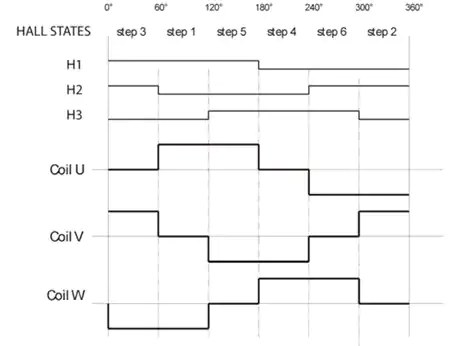
\includegraphics[width=\textwidth]{Bilder/test.png} 
% % % 		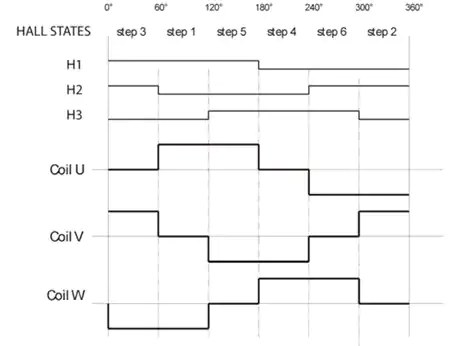
\includegraphics[width=100pt]{./Bilder/test.png}
% % % 		% \captionof{figure}[Beschleunigung und Verzögerung im v/t Diagramm]{Beschleunigung und Verzögerung im v/t Diagramm \label{v/t Diagramm}} 
% % % 		% \cite{Uebung1}
% % % 		% \captionsource{Caption}{Antriebstechnik Übung 1}
% \end{figure}

% \subsection{Dies ist eine Überschrift 2. Ordnung}
% Dies ist ein normaler Text in 10 pt Schrift-größe und 12 pt Zeilenabstand. Dies ist ein normaler Text in 10 pt Schriftgröße und 12 pt Zeilenabstand.
%  Dies ist ein normaler Text in 10 pt Schriftgröße und 12 pt Zeilen-abstand. Dies ist ein normaler Text in 10 pt Schriftgröße und 12 pt Zeilenabstand.normaler Text in 10 pt Schriftgröße und 12 pt Zeilenabstand. Dies ist ein normaler Text in 10 pt Schrift-größe und 12 pt Zeilenabstand. Dies ist ein normaler Text in 10 pt Schriftgröße und 12 pt Zeilenabstand. Dies ist ein normaler Text in 10 pt Schriftgröße und 12 pt Zeilen-abstand. Dies ist ein normaler Text in 10 pt Schriftgröße und 12 pt Zeilenabstand.normaler Text in 10 pt Schriftgröße und 12 pt Zeilenabstand.
% %\vfill				%Genaue Abtrennung nach diesem Wort
% %\columnbreak 		%Beginnt neue spalte
% Dies ist ein normaler Text in 10 pt Schrift-größe und 12 pt Zeilenabstand. Dies ist ein normaler Text in 10 pt Schriftgröße und 12 pt Zeilenabstand.
%  Dies ist ein normaler Text in 10 pt Schriftgröße und 12 pt Zeilen-abstand. Dies ist ein normaler Text in 10 pt Schriftgröße und 12 pt Zeilenabstand.normaler Text in 10 pt Schriftgröße und 12 pt Zeilenabstand. Dies ist ein normaler Text in 10 pt Schrift-größe und 12 pt Zeilenabstand. Dies ist ein normaler Text in 10 pt Schriftgröße und 12 pt Zeilenabstand.

% \subsubsection{Dies ist eine Überschrift 3. Ordnung}

%  Dies ist ein normaler Text in 10 pt Schriftgröße und 12 pt Zeilen-abstand. Dies ist ein normaler Text in 10 pt Schriftgröße und 12 pt Zeilenabstand.normaler Text in 10 pt Schriftgröße und 12 pt Zeilenabstand. Dies ist ein normaler Text in 10 pt Schrift-größe und 12 pt Zeilenabstand. Dies ist ein normaler Text in 10 pt Schriftgröße und 12 pt Zeilenabstand.
%  Dies ist ein normaler Text in 10 pt Schriftgröße und 12 pt Zeilen-abstand. Dies ist ein normaler Text in 10 pt Schriftgröße und 12 pt Zeilenabstand.normaler Text in 10 pt Schriftgröße und 12 pt Zeilenabstand. Dies ist ein normaler Text in 10 pt Schrift-größe und 12 pt Zeilenabstand. Dies ist ein normaler Text in 10 pt Schriftgröße und 12 pt Zeilenabstand.
%  Dies ist ein normaler Text in 10 pt Schriftgröße und 12 pt Zeilen-abstand. Dies ist ein normaler Text in 10 pt Schriftgröße und 12 pt Zeilenabstand.normaler Text in 10 pt Schriftgröße und 12 pt Zeilenabstand. Dies ist ein normaler Text in 10 pt Schrift-größe und 12 pt Zeilenabstand. Dies ist ein normaler Text in 10 pt Schriftgröße und 12 pt Zeilenabstand.
%  Dies ist ein normaler Text in 10 pt Schriftgröße und 12 pt Zeilen-abstand. Dies ist ein normaler Text in 10 pt Schriftgröße und 12 pt Zeilenabstand.normaler Text in 10 pt Schriftgröße und 12 pt Zeilenabstand. Dies ist ein normaler Text in 10 pt Schrift-größe und 12 pt Zeilenabstand. Dies ist ein normaler Text in 10 pt Schriftgröße und 12 pt Zeilenabstand.
%  Dies ist ein normaler Text in 10 pt Schriftgröße und 12 pt Zeilen-abstand. Dies ist ein normaler Text in 10 pt Schriftgröße und 12 pt Zeilenabstand.normaler Text in 10 pt Schriftgröße und 12 pt Zeilenabstand. Dies ist ein normaler Text in 10 pt Schrift-größe und 12 pt Zeilenabstand. Dies ist ein normaler Text in 10 pt Schriftgröße und 12 pt Zeilenabstand.
%  Dies ist ein normaler Text in 10 pt Schriftgröße und 12 pt Zeilen-abstand. Dies ist ein normaler Text in 10 pt Schriftgröße und 12 pt Zeilenabstand.normaler Text in 10 pt Schriftgröße und 12 pt Zeilenabstand. 


% $\rho = \frac{m}{V}$

% \begin{equation}
% {\rho = \frac{m}{V}}
% \end{equation}

% Dies ist ein normaler Text in 10 pt Schrift-größe und 12 pt Zeilenabstand. Dies ist ein normaler Text in 10 pt Schriftgröße und 12 pt Zeilenabstand.
%  Dies ist ein normaler Text in 10 pt Schriftgröße und 12 pt Zeilen-abstand. Dies ist ein normaler Text in 10 pt Schriftgröße und 12 pt Zeilenabstand.normaler Text in 10 pt Schriftgröße und 12 pt Zeilenabstand. Dies ist ein normaler Text in 10 pt Schrift-größe und 12 pt Zeilenabstand. Dies ist ein normaler Text in 10 pt Schriftgröße und 12 pt Zeilenabstand. 
 
% \paragraph{Dies ist eine Überschrift 4. Ordnung} $\;$\\%Trick zu Erzeugung eines Zeilenumbruchs
% Dies ist ein normaler Text in 10 pt Schriftgröße und 12 pt Zeilen-abstand. Dies ist ein normaler Text in 10 pt Schriftgröße und 12 pt Zeilenabstand.normaler Text in 10 pt Schriftgröße und 12 pt Zeilenabstand.Dies ist ein normaler Text in 10 pt Schriftgröße und 12 pt Zeilenabstandnormaler Text in 10 pt Schriftgröße und 12 pt Zeilenabstand.
	
	
% \noindent%
% \begin{minipage}{0.9\columnwidth}  %.9 auf 90 Prozent skaliert 
% \centering 
% \resizebox{0.9\columnwidth}{!} 
% 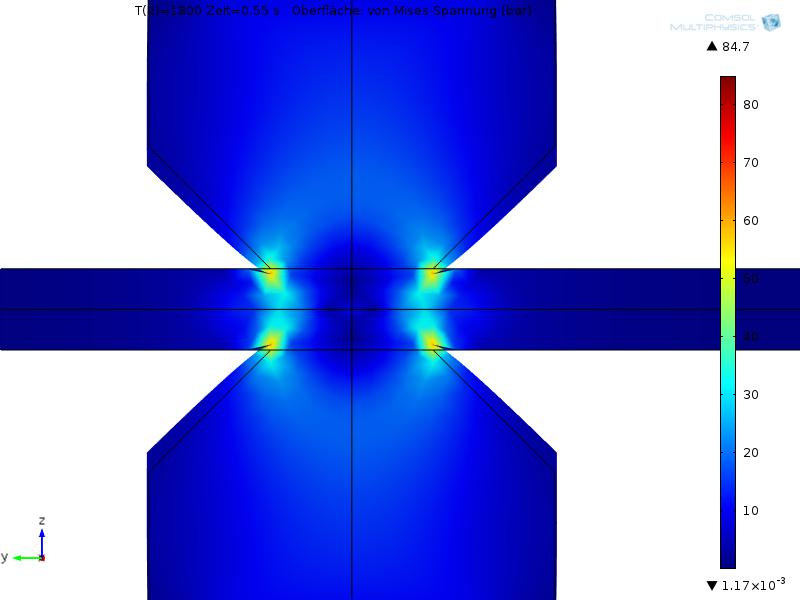
\includegraphics[width=\textwidth]{./Bilder/Testbild} 
% \captionof{figure}[Kurz-Caption]{Spannungsverlauf \label{caption}} 
% \end{minipage} 

% \vspace{4mm}

% \hspace{-4mm}
% Dies ist eine Referenz für Abbildung \ref{caption} normaler Text in 10 pt Schriftgröße und 12 pt Zeilenabstand.normaler Text in 10 pt Schriftgröße und 12 pt Zeilenabstand. Dies ist ein normaler Text in 10 pt Schriftgröße und 12 pt Zeilenabstand.normaler Text in 10 pt Schriftgröße und 12 pt Zeilenabstand. Dies ist ein normaler Text in 10 pt Schriftgröße und 12 pt Zeilenabstand.normaler Text in 10 pt Schriftgröße und 12 pt Zeilenabstand. Dies ist ein normaler Text in 10 pt Schriftgröße und 12 pt Zeilenabstand.normaler Text in 10 pt Schriftgröße und 12 pt Zeilenabstand. Dies ist ein normaler Text in 10 pt Schriftgröße und 12 pt Zeilenabstand.normaler Text in 10 pt Schriftgröße und 12 pt Zeilenabstand. Dies ist ein normaler Text in 10 pt Schriftgröße und 12 pt Zeilenabstand. Zitat
% \cite{AnalogDev} % Zitat
Dies ist ein normaler Text in 10 pt Schriftgröße und 12 pt Zeilenabstand.


\begin{thebibliography}{9}

\bibitem{Elko}
TDK-Lambda Germany GmbH [online], [Zugriff am 22.12.2021] Verfuegbar unter:	https://www.emea.lambda.tdk.com/de/KB/Was-Sie-über-die-Lebensdauer-von-Stromversorgungen-wissen-sollten.pdf
Aachen, TDK-Lambda Germany GmbH



\bibitem{Motor_Ansteuerung}
Steven Keeping: An Introduction to Brushless DC Motor Control, Digi-Key Electronics, 27.03.2013, Zugriff am 22.12.2021] Verfuegbar unter: https://www.digikey.de/de/articles/an-introduction-to-brushless-dc-motor-control

\bibitem{Leiterbahnbreite}
IPC  [online], [Zugriff am 22.12.2021] Verfuegbar unter https://www.ipc.org/TOC/IPC-2221.pdf, United States, IPC

\bibitem{PCB_Querschnitt}
Cree, Inc. Optimizing PCB Thermal Performance for Cree XLamp LEDs 22.12.2010, [Zugriff am 22.12.2021] Verfuegbar unter https://www.digikey.de/en/articles/optimizing-pcb-thermal-performance-for-cree-xlamp-leds

\bibitem{aisler}
Aisler B. V.  [online], [Zugriff am 22.12.2021] Verfuegbar unter https://aisler.net/help/design-rules-and-specifications/specifications












\bibitem{AnalogDev}
    Analog Devices: Analog Design		Seminar.
 	München: Analog Devices GmbH,
  	1989



\bibitem{Lancas86}
  	Lancaster, Don: Das Aktiv-			Filter-Kochbuch. Vaterstetten:  	IWT, 1986 

		
\bibitem{Gruetz97}
	Grütz, A.: Jahrbuch 				Elektrotechnik ’98. Berlin 			Offenbach: VDE-VERLAG, 				1997

\bibitem{Huneus91}
	H.; Lex, A.: Magnetische 			Eigenschaft von 					nichtkornorientiertem 				Elektroblech. etz Elektrotech. 	Z. 112 (1991) H. 22, S. 1204 – 	1208
	
\bibitem{Abramo80}
	Abramowitz, M.: Handbook of 		mathematical func-tions. 3. 			Aufl., New York: Dover, 1980
	
\bibitem{Elect97}
	Guidelines for ETEP-Authors. 		ETEP European Trans-actions on 	Electrical Power. Vol. 7, No. 		5, Sept./Oct. 1997, pp. 363 – 		364
  	
\end{thebibliography}

\end{multicols}
 

\end{document}
